\section{Struktur Dateisystem}
Die Struktur der Dateien ist klar getrennt (Abbildung \ref{fig:Ordnerstruktur}).
\begin{figure}[ !h] \centering
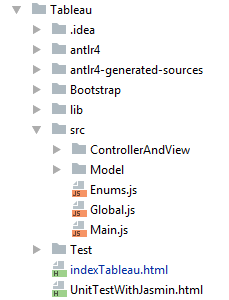
\includegraphics[]{Ordnerstruktur}
\caption[Ordnerstruktur]{Ordnerstruktur}\label{fig:Ordnerstruktur}
\end{figure}

In dem \textit{``Tableau''} Ordner liegen alle Dateien, welche in die Seite eingebunden werden. Dazu zählt ANTLR- und Bootstrap-Framework, generierte Dateien von ANTLR, Bibliothek, JavaSript Dateien und Test. Neben dem Ordner liegen weitere 
Html Dateien. Dazu zählt die 
%Dateien wie die statische Seite. Die Statische Seite ist eine einfache HTML-Datei 
\textit{``indexTableau.html''}, welche durch eingebundenes JavaScript interaktiv mit dem Anwender interagiert. Für das Testen des JavaScripts bietet es sich an, die HTML-Dateien \textit{``UnitTestModel.html''} und \textit{``UnitTestControllerView.html''}zu erstellen, die zusätzlich die Testfälle beinhaltet.

Der \textit{``antlr4-generated-soures''} Ordner (Abbildung \ref{fig:antlr4-generated-sources Ordner}) erhält die ANTLR-Runtime, BAT-Datei um die Runtime auszuführen, Grammatik der aussagenlogischen Formeln und alle Dateien wie  Token, Lexer, Parser, Listener und Visitor, welche die ANTLR-Runtime generiert hat.
\begin{figure}[ !h] \centering
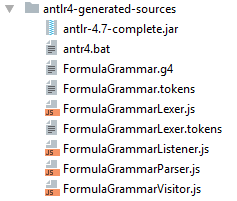
\includegraphics[]{antlr4GeneratedSources}
\caption[Ordnerstruktur antlr4GeneratedSources]{antlr4GeneratedSources}\label{fig:antlr4-generated-sources Ordner}
\end{figure}

Der \textit{``lib''} Ordner (Abbildung \ref{fig:libOrdner}) erhält die Jasmine-Bibliothek und \textit{``require.js''}.
\begin{figure}[ !h] \centering
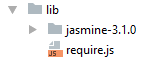
\includegraphics[]{lib}
\caption[Ordnerstruktur lib]{lib}\label{fig:libOrdner}
\vspace*{0.3cm}
\end{figure}

Für die Funktionalität der Webanwendung sorgen die JavaScript-Dateien aus dem \textit{``src''} Ordner (Abbildung \ref{fig:srcOrdner}). Dazu zählt das Model, Controller und View sowie alle Enumerationen, globale Variable und ``Namespaces''.
\begin{figure}[ !h] \centering
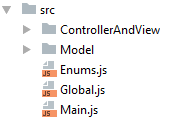
\includegraphics[]{src}
\caption[Ordnerstruktur src]{src}\label{fig:srcOrdner}
\vspace*{0.3cm}
\end{figure}

Zur Qualitätssicherung gibt es Unit-Tests. Diese liegen unterhalb des ``Tests'' Ordners (Abbildung \ref{fig:testOrdner}).
\begin{figure}[ !h] \centering
\includegraphics[]{test}
\caption[Ordnerstruktur test]{test}\label{fig:testOrdner}
\vspace*{0.3cm}
\end{figure}
